\documentclass[a4paper,twoside,openany]{../svmonoBUGS}\usepackage[]{graphicx}\usepackage[]{color}
% maxwidth is the original width if it is less than linewidth
% otherwise use linewidth (to make sure the graphics do not exceed the margin)
\makeatletter
\def\maxwidth{ %
  \ifdim\Gin@nat@width>\linewidth
    \linewidth
  \else
    \Gin@nat@width
  \fi
}
\makeatother

\definecolor{fgcolor}{rgb}{0.345, 0.345, 0.345}
\newcommand{\hlnum}[1]{\textcolor[rgb]{0.686,0.059,0.569}{#1}}%
\newcommand{\hlstr}[1]{\textcolor[rgb]{0.192,0.494,0.8}{#1}}%
\newcommand{\hlcom}[1]{\textcolor[rgb]{0.678,0.584,0.686}{\textit{#1}}}%
\newcommand{\hlopt}[1]{\textcolor[rgb]{0,0,0}{#1}}%
\newcommand{\hlstd}[1]{\textcolor[rgb]{0.345,0.345,0.345}{#1}}%
\newcommand{\hlkwa}[1]{\textcolor[rgb]{0.161,0.373,0.58}{\textbf{#1}}}%
\newcommand{\hlkwb}[1]{\textcolor[rgb]{0.69,0.353,0.396}{#1}}%
\newcommand{\hlkwc}[1]{\textcolor[rgb]{0.333,0.667,0.333}{#1}}%
\newcommand{\hlkwd}[1]{\textcolor[rgb]{0.737,0.353,0.396}{\textbf{#1}}}%
\let\hlipl\hlkwb

\usepackage{framed}
\makeatletter
\newenvironment{kframe}{%
 \def\at@end@of@kframe{}%
 \ifinner\ifhmode%
  \def\at@end@of@kframe{\end{minipage}}%
  \begin{minipage}{\columnwidth}%
 \fi\fi%
 \def\FrameCommand##1{\hskip\@totalleftmargin \hskip-\fboxsep
 \colorbox{shadecolor}{##1}\hskip-\fboxsep
     % There is no \\@totalrightmargin, so:
     \hskip-\linewidth \hskip-\@totalleftmargin \hskip\columnwidth}%
 \MakeFramed {\advance\hsize-\width
   \@totalleftmargin\z@ \linewidth\hsize
   \@setminipage}}%
 {\par\unskip\endMakeFramed%
 \at@end@of@kframe}
\makeatother

\definecolor{shadecolor}{rgb}{.97, .97, .97}
\definecolor{messagecolor}{rgb}{0, 0, 0}
\definecolor{warningcolor}{rgb}{1, 0, 1}
\definecolor{errorcolor}{rgb}{1, 0, 0}
\newenvironment{knitrout}{}{} % an empty environment to be redefined in TeX

\usepackage{alltt}
\title{Bayesian methods in health economics \\ STAT3021/STATM021/STATG021}
\author{Practicals}
\date{January -- March 2018}

\usepackage{xspace,graphicx,bm,amssymb,amsmath,url,graphics,inconsolata}
\usepackage[text={15.2cm,22cm},centering]{geometry}
\usepackage{inconsolata}
\usepackage[T1]{fontenc}
\usepackage[normalem]{ulem}
\usepackage{charter}
\usepackage{tikz,verbatim,graphicx,color}
%%%\usetikzlibrary{shapes,arrows,arrows.meta,decorations.pathreplacing,shapes.geometric}


\newcommand{\winbugs}{{\texttt{WinBUGS}}\xspace}
\newcommand{\openbugs}{{\texttt{OpenBUGS}}\xspace}
\newcommand{\jags}{{\texttt{JAGS}}\xspace}
\newcommand{\bugs}{{\texttt{BUGS}}\xspace}
\newcommand{\R}{{\texttt{R}}\xspace}
\newcommand{\bcea}{{\texttt{BCEA}}\xspace}

\usepackage{listings}
\lstset{basicstyle=\ttfamily\fontsize{9}{11}\selectfont,breaklines=true,tabsize=2,
keywords={},linewidth=1\textwidth,backgroundcolor=\color{black!5}} 

\renewcommand{\chaptername}{Practical}

\graphicspath{{/home/gianluca/Dropbox/EcSan/ShortCourses/BSU-UCL/LaTeX/}{/home/gianluca/Dropbox/UCL/3021/Lectures/figs/}}
\IfFileExists{upquote.sty}{\usepackage{upquote}}{}
\begin{document}
\addtocounter{chapter}{7}
\chapter{Introduction to Markov models --- SOLUTIONS}


\section{Simple model}
Consider a three-state model is used to describe how patients transition between health states with a chronic disease.
Patients begin in an asymptomatic health state, which means that the patient has developed the chronic disease but has so symptoms.
Patients can stay in the asymptomatic health state or move to a progressive health state which means that the patient is experiencing symptoms of the disease.
Patients can move from the asymptomatic health state to the dead health state at the same rate as the general population without the disease.
Patients can stay in the progressive health state or move from the progressive health state to dead, but at an increased risk of death.
The dead state is an absorbing state as a patient cannot change from being dead.

\begin{figure}
\centering
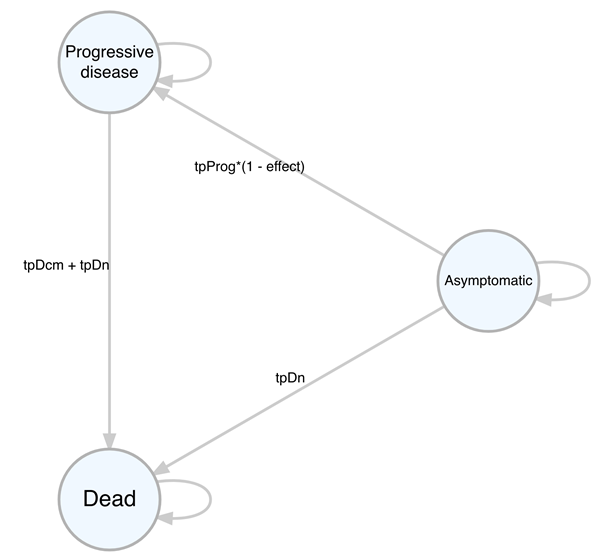
\includegraphics[scale=1]{model-diagram}
\end{figure}

A cohort of 1000 patients receives a drug and compares to a cohort of 1000 patients that does not receive a drug to assess how patients move throughout the health states over time with a chronic disease. To set up thel model in R some definitions are needed first. We outline the R code used to define the number of treatments (prefixed with \texttt{t\_}) and their names (prefixed with \texttt{n\_}), the number of states (prefixed with \texttt{s\_}) and their names. The number of cycles starting at 1 (not 0 as in spreadsheet models) is specified, as well as the initial age of patients in the cohort beginning at 55.

\begin{verbatim}
## model set-up ----

t_names <- c("without_drug", "with_drug")
n_treatments <- length(t_names)

s_names  <- c("Asymptomatic_disease", "Progressive_disease", "Dead")
n_states <- length(s_names)

n_pop <- 1000

n_cycles <- 46
Initial_age <- 55
\end{verbatim}

The unit costs and unit utilities associated with each of the health states as well as the cost of the drug need to be defined.
The utility of being in the dead health state is 0 so does not need to be defined here.
Costs begin with a c and utilities with a u. The discount rate for costs and outcomes are also included at a rate of 6\%.
The probability of dying from the disease in a single cycle (tpDcm) is now defined.

\begin{verbatim}
cAsymp <- 500
cDeath <- 1000
cDrug <- 1000
cProg <- 3000
uAsymp <- 0.95
uProg <- 0.75
oDr <- 0.06
cDr <- 0.06
tpDcm <- 0.15

# transition matrix variables
tpProg <- 0.01
tpDcm <- 0.15
tpDn <- 0.0138
effect <- 0.5
\end{verbatim}

This process of defining treatment names, states and cycles is similar to that in MS Excel. One addition in R is that space for when calculations are performed is needed. It is like creating the cells in MS Excel. By creating matrices, empty space for costs and utilities in each health state for patients with or without the drug is specified. The structure of the matrices for the cost of transition to a health state, and cost and QALYs accrued being in health state are the same. We describe the cost of transitioning to a state, in this case only for the dead state. The first argument defines a vector of values for each health state and for each cohort, similar to a column of values in a parameters sheet in Excel. The argument \texttt{byrow = TRUE} makes sure that all the states for the first cohort are defined first and then all the states for the second cohort.
The \texttt{trans\_c\_matrix} creates empty space and assigned the cost of £1000 for transitioning to the Dead state.
The first line is for the cohort who are without a drug, and the second line for the cohort that are with a drug. 

\begin{verbatim}
# cost of staying in state
state_c_matrix <-
  matrix(c(cAsymp, cProg, 0,
           cAsymp + cDrug, cProg, 0),
         byrow = TRUE,
         nrow = n_treatments,
         dimnames = list(t_names,
                         s_names))

# qaly when staying in state
state_q_matrix <-
  matrix(c(uAsymp, uProg, 0,
           uAsymp, uProg, 0),
         byrow = TRUE,
         nrow = n_treatments,
         dimnames = list(t_names,
                         s_names))

# cost of moving to a state
# same for both treatments
trans_c_matrix <-
  matrix(c(0, 0, 0,
           0, 0, cDeath,
           0, 0, 0),
         byrow = TRUE,
         nrow = n_states,
         dimnames = list(from = s_names,
                         to = s_names))
\end{verbatim}

The probability of dying from the disease in a single cycle (tpDcm) was defined above. Space is also needed to define the transition probabilities between health states. A matrix is created as above but with another dimension for the movements between health states. The resulting matrix shows an empty space for the transitions between each health state dependent on the cohort being with or without a drug.

\begin{itemize}
\item The reason that they are in this order is because when printed out then the square matrix is preserved so we can see from which state to which state. The array is split by the third dimension treatment.
\end{itemize}

\begin{verbatim}
# Transition probabilities
p_matrix <- array(data = 0,
                  dim = c(n_states, n_states, n_treatments),
                  dimnames = list(from = s_names,
                                  to = s_names,
                                  t_names))

## assume doesn't depend on cycle
p_matrix["Asymptomatic_disease", "Progressive_disease", "without_drug"] <- tpProg
p_matrix["Asymptomatic_disease", "Dead", "without_drug"] <- tpDn
p_matrix["Asymptomatic_disease", "Asymptomatic_disease", "without_drug"] <- 1 - tpProg - tpDn
p_matrix["Progressive_disease", "Dead", "without_drug"] <- tpDcm + tpDn
p_matrix["Progressive_disease", "Progressive_disease", "without_drug"] <- 1 - tpDcm - tpDn
p_matrix["Dead", "Dead", "without_drug"] <- 1

# Matrix containing transition probabilities for with_drug
p_matrix["Asymptomatic_disease", "Progressive_disease", "with_drug"] <- tpProg*(1 - effect)
p_matrix["Asymptomatic_disease", "Dead", "with_drug"] <- tpDn
p_matrix["Asymptomatic_disease", "Asymptomatic_disease", "with_drug"] <- 1 - tpProg*(1 - effect) - tpDn
p_matrix["Progressive_disease", "Dead", "with_drug"] <- tpDcm + tpDn
p_matrix["Progressive_disease", "Progressive_disease", "with_drug"] <- 1 - tpDcm - tpDn
p_matrix["Dead", "Dead", "with_drug"] <- 1

# Store population output for each cycle 

# state populations
pop <- array(data = NA,
             dim = c(n_states, n_cycles, n_treatments),
             dimnames = list(state = s_names,
                             cycle = NULL,
                             treatment = t_names))

pop["Asymptomatic_disease", cycle = 1, ] <- n_pop
pop["Progressive_disease", cycle = 1, ] <- 0
pop["Dead", cycle = 1, ] <- 0
\end{verbatim}

\begin{itemize}
\item Theres no need to specify each treatment separately. Simply leave the last dimension empty and it will replicate the value for all treatments.
\end{itemize}

\begin{verbatim}
# _arrived_ state populations
trans <- array(data = NA,
               dim = c(n_states, n_cycles, n_treatments),
               dimnames = list(state = s_names,
                               cycle = NULL,
                               treatment = t_names))

trans[, cycle = 1, ] <- 0
\end{verbatim}

\section{Output Variables}
A population matrix (\texttt{pop}) and transition matrix (\texttt{trans}) are created with an additional dimension so there is blank space for each health state, with or without a drug, for each of the 46 cycles. Below shows this process for a generic array (\texttt{cycle\_empty\_array}).

\begin{verbatim}
# Sum costs and QALYs for each cycle at a time for each drug 

cycle_empty_array <-
  array(NA,
        dim = c(n_treatments, n_cycles),
        dimnames = list(treatment = t_names,
                        cycle = NULL))

cycle_state_costs <- cycle_trans_costs <- cycle_empty_array
cycle_costs <- cycle_QALYs <- cycle_empty_array
LE <- LYs <- cycle_empty_array    # life-expectancy; life-years
cycle_QALE <- cycle_empty_array   # qaly-adjusted life-years

total_costs <- setNames(c(NA, NA), t_names)
total_QALYs <- setNames(c(NA, NA), t_names)
\end{verbatim}

\section{Running the model}
To run the model and combine all the information and code from the previous sections, an algorithm will be created.
A loop is first created over treatments and then a second loop repeats from cycle number 2 to cycle 46 (\texttt{n\_cycles}), as cycle 1 was already defined above, equivalent to cycle 0 rows in Excel models. Recall the matrix multiplication operator \texttt{\%*\%}, used here to calculate the state population at the next time step (\texttt{pop}) and the number of individuals who transition between states (\texttt{trans}).

\begin{verbatim}
for (i in 1:n_treatments) {
  
  age <- Initial_age
  
  for (j in 2:n_cycles) {
    
    pop[, cycle = j, treatment = i] <-
      pop[, cycle = j - 1, treatment = i] %*% p_matrix[, , treatment = i]
    
    trans[, cycle = j, treatment = i] <-
      pop[, cycle = j - 1, treatment = i] %*% (trans_c_matrix * p_matrix[, , treatment = i])
    
    age <- age + 1
  }
  
  cycle_state_costs[i, ] <-
    (state_c_matrix[treatment = i, ] %*% pop[, , treatment = i]) * 1/(1 + cDr)^(1:n_cycles - 1)
  
  # discounting at _previous_ cycle
  cycle_trans_costs[i, ] <-
    (c(1,1,1) %*% trans[, , treatment = i]) * 1/(1 + cDr)^(1:n_cycles - 2)
  
  cycle_costs[i, ] <- cycle_state_costs[i, ] + cycle_trans_costs[i, ]
  
  LE[i, ] <- c(1,1,0) %*% pop[, , treatment = i]
  
  LYs[i, ] <- LE[i, ] * 1/(1 + oDr)^(1:n_cycles - 1)
  
  cycle_QALE[i, ] <-
    state_q_matrix[treatment = i, ] %*% pop[, , treatment = i]
  
  cycle_QALYs[i, ] <- cycle_QALE[i, ] * 1/(1 + oDr)^(1:n_cycles - 1)
  
  total_costs[i] <- sum(cycle_costs[treatment = i, -1])
  total_QALYs[i] <- sum(cycle_QALYs[treatment = i, -1])
}
\end{verbatim}
The discount rate is also incorporated into the model here easily as each cycle’s costs and QALYs will depend on the cycle number. These repeated steps are performed for each of the two treatments (1:n treatments) and the total costs and QALYs over the lifetime of the model can then be calculated for each treatment.

%
\section{Plot results}
Displaying the results after running the model is easy in \R. . These results will therefore assume that the strategy where the cohort are without a drug is the standard of care or base case analysis. Swapping with and without the drug will change this around.

\begin{verbatim}
# Incremental costs and QALYs of with_drug vs to without_drug
c_incr <- total_costs["with_drug"] - total_costs["without_drug"]
q_incr <- total_QALYs["with_drug"] - total_QALYs["without_drug"]

# Incremental cost effectiveness ratio 
ICER <- c_incr/q_incr
\end{verbatim}

Create a simple cost-effectiveness plane as follows:

\begin{verbatim}
plot(x = q_incr/n_pop, y = c_incr/n_pop,
     xlim = c(0, 1500/n_pop),
     ylim = c(0, 12e6/n_pop),
     pch = 16, cex = 1.5,
     xlab = "QALY difference",
     ylab = "Cost difference (£)",
     frame.plot = FALSE)
\end{verbatim}

The point is below the threshold and so the new drug is cost-effective.

%
\section{Cycle-dependent probability matrix}
Transition probabilities in a Markov model can either be time-independent, such as tpDm, or time-dependent.
Next, define the transition probabilities in the full model depend on age and cycle.
To begin with let us only depend on cycle and fix the age varying variable \texttt{tpDn} at a middle value.
Define the transition probability from Asymptomatic to Progressive disease, previously just \texttt{tpProg}, to depend on cycle such that the new transition probability is \texttt{tpProg} $\times$ \texttt{cycle}.

To account for the time dependency, the hard-coded array in MS Excel has been replaced with a function in R named \texttt{p\_matrix\_cycle} which is called at each cycle iteration. By simply replacing a fixed array with a function, this will decouple the calculation of the transition matrix and the higher-level cost-effectiveness calculations. This makes changes and testing to either part easier and more reliable.

Note that, strictly speaking, in R this is an array but we have named the data structure \texttt{p\_matrix} to emphasise that it provides what is known in Markov modelling as the transition probability matrix. The time dependent probabilities are those that depend on the age of the cohort. A lookup function is used to describe the transition probability from Asymp to Dead using 6 age group categories.

\begin{verbatim}
p_matrix_cycle <- function(p_matrix, cycle,
                           tpProg = 0.01,
                           tpDcm = 0.15,
                           tpDn = 0.0138
                           effect = 0.5) {
  
  # Matrix containing transition probabilities for without_drug
  p_matrix["Asymptomatic_disease", "Progressive_disease", "without_drug"] <- tpProg*cycle
  p_matrix["Asymptomatic_disease", "Dead", "without_drug"] <- tpDn
  p_matrix["Asymptomatic_disease", "Asymptomatic_disease", "without_drug"] <- 1 - tpProg*cycle - tpDn
  p_matrix["Progressive_disease", "Dead", "without_drug"] <- tpDcm + tpDn
  p_matrix["Progressive_disease", "Progressive_disease", "without_drug"] <- 1 - tpDcm - tpDn
  p_matrix["Dead", "Dead", "without_drug"] <- 1
  
  # Matrix containing transition probabilities for with_drug
  p_matrix["Asymptomatic_disease", "Progressive_disease", "with_drug"] <- tpProg*(1 - effect)*cycle
  p_matrix["Asymptomatic_disease", "Dead", "with_drug"] <- tpDn
  p_matrix["Asymptomatic_disease", "Asymptomatic_disease", "with_drug"] <-
    1 - tpProg*(1 - effect)*cycle - tpDn
  p_matrix["Progressive_disease", "Dead", "with_drug"] <- tpDcm + tpDn
  p_matrix["Progressive_disease", "Progressive_disease", "with_drug"] <- 1 - tpDcm - tpDn
  p_matrix["Dead", "Dead", "with_drug"] <- 1

  return(p_matrix)
}
\end{verbatim}


\section{Running the model}
The model is run in the same way as the first example.

\begin{verbatim}
for (i in 1:n_treatments) {
  
  age <- Initial_age
  
  for (j in 2:n_cycles) {
    
    p_matrix <- p_matrix_cycle(p_matrix, j - 1)
    
    pop[, cycle = j, treatment = i] <-
      pop[, cycle = j - 1, treatment = i] %*% p_matrix[, , treatment = i]
    
    trans[, cycle = j, treatment = i] <-
      pop[, cycle = j - 1, treatment = i] %*% (trans_c_matrix * p_matrix[, , treatment = i])
    
    age <- age + 1
  }
  
  cycle_state_costs[i, ] <-
    (state_c_matrix[treatment = i, ] %*% pop[, , treatment = i]) * 1/(1 + cDr)^(1:n_cycles - 1)
  
  # discounting at _previous_ cycle
  cycle_trans_costs[i, ] <-
    (c(1,1,1) %*% trans[, , treatment = i]) * 1/(1 + cDr)^(1:n_cycles - 2)
  
  cycle_costs[i, ] <- cycle_state_costs[i, ] + cycle_trans_costs[i, ]
  
  LE[i, ] <- c(1,1,0) %*% pop[, , treatment = i]
  
  LYs[i, ] <- LE[i, ] * 1/(1 + oDr)^(1:n_cycles - 1)
  
  cycle_QALE[i, ] <-
    state_q_matrix[treatment = i, ] %*% pop[, , treatment = i]
  
  cycle_QALYs[i, ] <- cycle_QALE[i, ] * 1/(1 + oDr)^(1:n_cycles - 1)
  
  total_costs[i] <- sum(cycle_costs[treatment = i, -1])
  total_QALYs[i] <- sum(cycle_QALYs[treatment = i, -1])
}
\end{verbatim}

The cost, QALY, LE, LY and QALE at each cycle are calculated as the \texttt{p\_matrix} is updated at each iteration of the loop.



\section{Plot results}

\begin{verbatim}
# Incremental costs and QALYs of with_drug vs to without_drug
c_incr <- total_costs["with_drug"] - total_costs["without_drug"]
q_incr <- total_QALYs["with_drug"] - total_QALYs["without_drug"]

# Incremental cost effectiveness ratio 
ICER <- c_incr/q_incr
\end{verbatim}

\begin{verbatim}
plot(x = q_incr/n_pop, y = c_incr/n_pop,
     xlim = c(0, 1500/n_pop),
     ylim = c(0, 12e6/n_pop),
     pch = 16, cex = 1.5,
     xlab = "QALY difference",
     ylab = "Cost difference (£)",
     frame.plot = FALSE)
\end{verbatim}

The point is further to the right and lower meaning it is less costly and more effective than in the previous analysis.


\section{Age-dependent probability matrix}
Now extend the \texttt{p\_matrix\_cycle()} function to include a dependence on age as well as cycle.
The additional code looks like the following:

\begin{verbatim}
p_matrix_cycle <- function(p_matrix, age, cycle,
                           tpProg = 0.01,
                           tpDcm = 0.15,
                           effect = 0.5) {
  
 # time-dependent age lookup table
  tpDn_lookup <-
    c("(34,44]" = 0.0017,
      "(44,54]" = 0.0044,
      "(54,64]" = 0.0138,
      "(64,74]" = 0.0379,
      "(74,84]" = 0.0912,
      "(84,100]" = 0.1958)
  
  # discretize age in to age groups
  age_grp <- cut(age, breaks = c(34,44,54,64,74,84,100))
  
  # map an age group to a probability
  tpDn <- tpDn_lookup[age_grp]
  
  # Matrix containing transition probabilities for without_drug
  
  p_matrix["Asymptomatic_disease", "Progressive_disease", "without_drug"] <- tpProg*cycle
  p_matrix["Asymptomatic_disease", "Dead", "without_drug"] <- tpDn
  p_matrix["Asymptomatic_disease", "Asymptomatic_disease", "without_drug"] <- 1 - tpProg*cycle - tpDn
  p_matrix["Progressive_disease", "Dead", "without_drug"] <- tpDcm + tpDn
  p_matrix["Progressive_disease", "Progressive_disease", "without_drug"] <- 1 - tpDcm - tpDn
  p_matrix["Dead", "Dead", "without_drug"] <- 1
  
  # Matrix containing transition probabilities for with_drug
  p_matrix["Asymptomatic_disease", "Progressive_disease", "with_drug"] <- tpProg*(1 - effect)*cycle
  p_matrix["Asymptomatic_disease", "Dead", "with_drug"] <- tpDn
  p_matrix["Asymptomatic_disease", "Asymptomatic_disease", "with_drug"] <-
    1 - tpProg*(1 - effect)*cycle - tpDn
  p_matrix["Progressive_disease", "Dead", "with_drug"] <- tpDcm + tpDn
  p_matrix["Progressive_disease", "Progressive_disease", "with_drug"] <- 1 - tpDcm - tpDn
  p_matrix["Dead", "Dead", "with_drug"] <- 1
  
  return(p_matrix)
}
\end{verbatim}

To run the model use the following.

\begin{verbatim}

for (i in 1:n_treatments) {
  
  age <- Initial_age
  
  for (j in 2:n_cycles) {
    
    p_matrix <- p_matrix_cycle(p_matrix, age, j - 1)
    
    pop[, cycle = j, treatment = i] <-
      pop[, cycle = j - 1, treatment = i] %*% p_matrix[, , treatment = i]
    
    trans[, cycle = j, treatment = i] <-
      pop[, cycle = j - 1, treatment = i] %*% (trans_c_matrix * p_matrix[, , treatment = i])
    
    age <- age + 1
  }
  
  cycle_state_costs[i, ] <-
    (state_c_matrix[treatment = i, ] %*% pop[, , treatment = i]) * 1/(1 + cDr)^(1:n_cycles - 1)
  
  # discounting at _previous_ cycle
  cycle_trans_costs[i, ] <-
    (c(1,1,1) %*% trans[, , treatment = i]) * 1/(1 + cDr)^(1:n_cycles - 2)
  
  cycle_costs[i, ] <- cycle_state_costs[i, ] + cycle_trans_costs[i, ]
  
  LE[i, ] <- c(1,1,0) %*% pop[, , treatment = i]
  
  LYs[i, ] <- LE[i, ] * 1/(1 + oDr)^(1:n_cycles - 1)
  
  cycle_QALE[i, ] <-
    state_q_matrix[treatment = i, ] %*% pop[, , treatment = i]
  
  cycle_QALYs[i, ] <- cycle_QALE[i, ] * 1/(1 + oDr)^(1:n_cycles - 1)
  
  total_costs[i] <- sum(cycle_costs[treatment = i, -1])
  total_QALYs[i] <- sum(cycle_QALYs[treatment = i, -1])
}


## Plot results ----

# Incremental costs and QALYs of with_drug vs to without_drug
c_incr <- total_costs["with_drug"] - total_costs["without_drug"]
q_incr <- total_QALYs["with_drug"] - total_QALYs["without_drug"]

## what the incremental cost effectiveness ratio?
ICER <- 
  
  plot(x = q_incr/n_pop, y = c_incr/n_pop,
       xlim = c(0, 1500/n_pop),
       ylim = c(0, 12e6/n_pop),
       pch = 16, cex = 1.5,
       xlab = "QALY difference",
       ylab = "Cost difference (£)",
       frame.plot = FALSE)
abline(a = 0, b = 30000) # Willingness-to-pay threshold
\end{verbatim}

The point is closer to the origin. It slightly less costly and less effective than the previous analysis.


\section{Probability Sensitivity Analysis (PSA)}
The formulation in the previous section can be extended to include uncertainty about one or more of the parameters. Briggs (2000) describe this for the current model by repeating the analytical solution of the model employing different values for the underlying parameters sampled from specified ranges and distributions. Sensitivity analyses can be performed one at a time (one-way) or for multiple parameters simultaneously (multi-way). This section presents a multi-way probabilistic sensitivity analysis. 

Performing a PSA analysis can be done by inputting random draws from the unit costs and QALY distributions as inputs to the existing model function. In R, there are numerous ways of implementing a PSA. Following from the R code presented in the previous sections, we can wrap this model code in a function, e.g. called \texttt{ce\_markov()}, which we can then repeatedly call with different parameter values. To this we will need to pass the starting conditions: population (\texttt{start\_pop}), age (\texttt{init\_age}) and number of cycles (\texttt{n\_cycle}) (in our case, if not defined then age and number of cycles are assigned default values). We will also need the probability transition matrix \texttt{(p\_matrix}), state cost and QALY matrices (\texttt{state\_c\_matrix}, \texttt{state\_q\_matrix}, \texttt{trans\_c\_matrix}).

In extension to the first analysis, the unit values have distributions rather than point values. To sample from a base R distribution the function name syntax is a short form version of the distribution name preceded by and \texttt{r} (for random or realisation). For example, to sample from a normal distribution then call \texttt{rnorm()}. We could sample all of the random numbers before running the model which would allow us to save them to use again and improve run time because this would only be performed once outside of the main loop. Alternatively, we can sample the random variables at runtime, within the Markov model function. This is arguably neater and if we wish to replicate a particular run then we can set the random seed beforehand with \texttt{set.seed()}. We will demonstrate how to implement a simple version when sampling at runtime.


\begin{verbatim}
ce_markov <- function(start_pop,
                      p_matrix,
                      state_c_matrix,
                      trans_c_matrix,
                      state_q_matrix,
                      n_cycles = 46,
                      init_age = 55,
                      s_names = NULL,
                      t_names = NULL) {
  
  n_states <- length(start_pop)
  n_treat <- dim(p_matrix)[3]
  
  pop <- array(data = NA,
               dim = c(n_states, n_cycles, n_treat),
               dimnames = list(state = s_names,
                               cycle = NULL,
                               treatment = t_names))
  trans <- array(data = NA,
                 dim = c(n_states, n_cycles, n_treat),
                 dimnames = list(state = s_names,
                                 cycle = NULL,
                                 treatment = t_names))
  
  for (i in 1:n_states) {
    pop[i, cycle = 1, ] <- start_pop[i]
  }

  cycle_empty_array <-
    array(NA,
          dim = c(n_treat, n_cycles),
          dimnames = list(treatment = t_names,
                          cycle = NULL))
  
  cycle_state_costs <- cycle_trans_costs <- cycle_empty_array
  cycle_costs <- cycle_QALYs <- cycle_empty_array
  LE <- LYs <- cycle_empty_array    # life-expectancy; life-years
  cycle_QALE <- cycle_empty_array   # qaly-adjusted life-years
  
  total_costs <- setNames(rep(NA, n_treat), t_names)
  total_QALYs <- setNames(rep(NA, n_treat), t_names)
  
  for (i in 1:n_treat) {
    
    age <- init_age
    
    for (j in 2:n_cycles) {
      
      # difference from point estimate case
      # pass in functions for random sample
      # rather than fixed values
      p_matrix <- p_matrix_cycle(p_matrix, age, j - 1,
                                 tpProg = tpProg(),
                                 tpDcm = tpDcm(),
                                 effect = effect())
      
      # Matrix multiplication
      pop[, cycle = j, treatment = i] <-
        pop[, cycle = j - 1, treatment = i] %*% p_matrix[, , treatment = i]
      
      trans[, cycle = j, treatment = i] <-
        pop[, cycle = j - 1, treatment = i] %*% (trans_c_matrix * p_matrix[, , treatment = i])
      
      age <- age + 1
    }
    
    cycle_state_costs[i, ] <-
      (state_c_matrix[treatment = i, ] %*% pop[, , treatment = i]) * 1/(1 + cDr)^(1:n_cycles - 1)
    
    cycle_trans_costs[i, ] <-
      (c(1,1,1) %*% trans[, , treatment = i]) * 1/(1 + cDr)^(1:n_cycles - 2)
    
    cycle_costs[i, ] <- cycle_state_costs[i, ] + cycle_trans_costs[i, ]
    
    LE[i, ] <- c(1,1,0) %*% pop[, , treatment = i]
    
    LYs[i, ] <- LE[i, ] * 1/(1 + oDr)^(1:n_cycles - 1)
    
    cycle_QALE[i, ] <-
     state_q_matrix[treatment = i, ] %*%  pop[, , treatment = i]
    
    cycle_QALYs[i, ] <- cycle_QALE[i, ] * 1/(1 + oDr)^(1:n_cycles - 1)
    
    total_costs[i] <- sum(cycle_costs[treatment = i, -1])
    total_QALYs[i] <- sum(cycle_QALYs[treatment = i, -1])
  }
  
  list(pop = pop,
       cycle_costs = cycle_costs,
       cycle_QALYs = cycle_QALYs,
       total_costs = total_costs,
       total_QALYs = total_QALYs)
}
\end{verbatim}

Because we will want to sample more than once, rather than just once at the start of the simulation, we can wrap the random sampling statements in a function so that they are called newly every time the Markov model is run. So, using the same names as we used for the point values in the previous analysis

\begin{verbatim}
# replace point values with functions to random sample

cAsymp <- function() rnorm(1, 500, 127.55)
cDeath <- function() rnorm(1, 1000, 255.11)
cDrug  <- function() rnorm(1, 1000, 102.04)
cProg  <- function() rnorm(1, 3000, 510.21)
effect <- function() rnorm(1, 0.5, 0.051)
tpDcm  <- function() rbeta(1, 29, 167)
tpProg <- function() rbeta(1, 15, 1506)
uAsymp <- function() rbeta(1, 69, 4)
uProg  <- function() rbeta(1, 24, 8)
\end{verbatim}

Similarly, rather than using fixed \texttt{state\_c\_matrix}, \texttt{trans\_c\_matrix} and \texttt{state\_q\_matrix}, if we define these as functions, we can sample newly their component values each time they are called. In practice, the code looks the same as previously but now the unit values are function calls so are followed by open and closed brackets. 

\begin{verbatim}
# Define cost and QALYs as functions

state_c_matrix <- function() {
  matrix(c(cAsymp(), cProg(), 0,            # without drug
           cAsymp() + cDrug(), cProg(), 0), # with drug
           byrow = TRUE,
           nrow = n_treatments,
           dimnames = list(t_names,
                           s_names))
}

state_q_matrix <- function() {
  matrix(c(uAsymp(), uProg(), 0,  # without drug
           uAsymp(), uProg(), 0), # with drug
         byrow = TRUE,
         nrow = n_treatments,
         dimnames = list(t_names,
                         s_names))
}

trans_c_matrix <- function() {
  matrix(c(0, 0, 0,         # Asymptomatic_disease
           0, 0, cDeath(),  # Progressive_disease
           0, 0, 0),        # Dead
         byrow = TRUE,
         nrow = n_states,
         dimnames = list(from = s_names,
                         to = s_names))
}
\end{verbatim}

\subsection{ Run PSA analysis}
To finally obtain the PSA output, loop over \texttt{ce\_markov()} remembering to record the cost and QALYs outputs each time.

\begin{verbatim}
n_trials <- 500

costs <- matrix(NA, nrow = n_trials, ncol = n_treatments,
                dimnames = list(NULL, t_names))
qalys <- matrix(NA, nrow = n_trials, ncol = n_treatments,
                dimnames = list(NULL, t_names))

for (i in 1:n_trials) {
  ce_res <- ce_markov(start_pop = c(n_pop, 0, 0),
                      p_matrix,
                      state_c_matrix(),
                      trans_c_matrix(),
                      state_q_matrix())
  
  costs[i, ] <- ce_res$total_costs
  qalys[i, ] <- ce_res$total_QALYs
}
\end{verbatim}



\subsection{Plot results}
We can use the same code as before because R is vectorised.

\begin{verbatim}
# incremental costs and QALYs of with_drug vs to without_drug
c_incr_psa <- costs[, "with_drug"] - costs[, "without_drug"]
q_incr_psa <- qalys[, "with_drug"] - qalys[, "without_drug"]

plot(x = q_incr_psa/n_pop, y = c_incr_psa/n_pop,
     xlim = c(0, 2),
     ylim = c(0, 15e3),
     pch = 16, cex = 1.2,
     col = "grey",
     xlab = "QALY difference",
     ylab = "Cost difference (£)",
     frame.plot = FALSE)
abline(a = 0, b = 30000, lwd = 2) # Willingness-to-pay threshold £30,000/QALY

points(x = q_incr/n_pop, y = c_incr/n_pop,
       col = "red",
       pch = 16, cex = 1.5)
\end{verbatim}

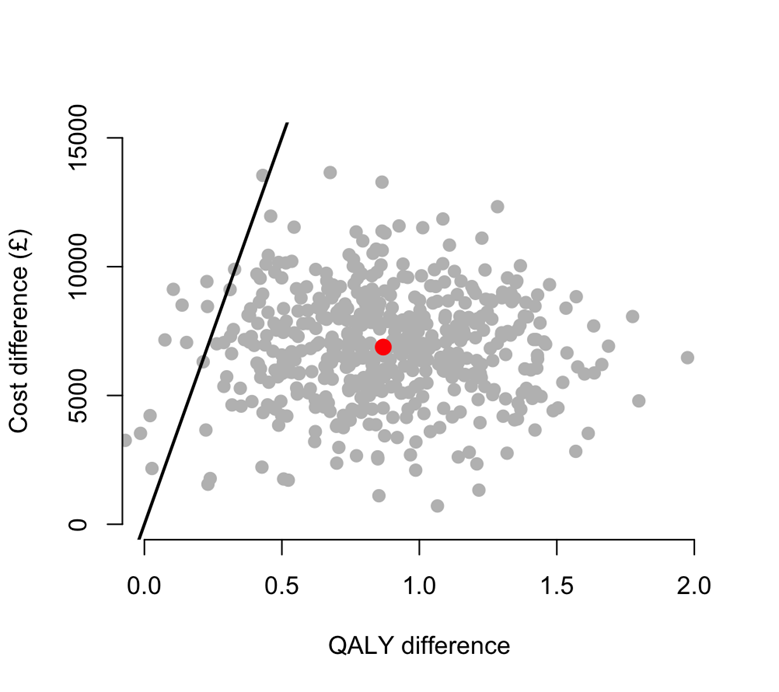
\includegraphics[scale=1]{ceplane_psa}

\begin{verbatim}
##########
## BCEA

library(BCEA)

mm_bcea <- bcea(qalys/n_pop, costs/n_pop, ref = 2,
                interventions = c("without_drug", "with_drug"))

ceplane.plot(mm_bcea)
ceac.plot(mm_bcea, graph = "ggplot2")
eib.plot(mm_bcea)
summary(mm_bcea)
\end{verbatim}

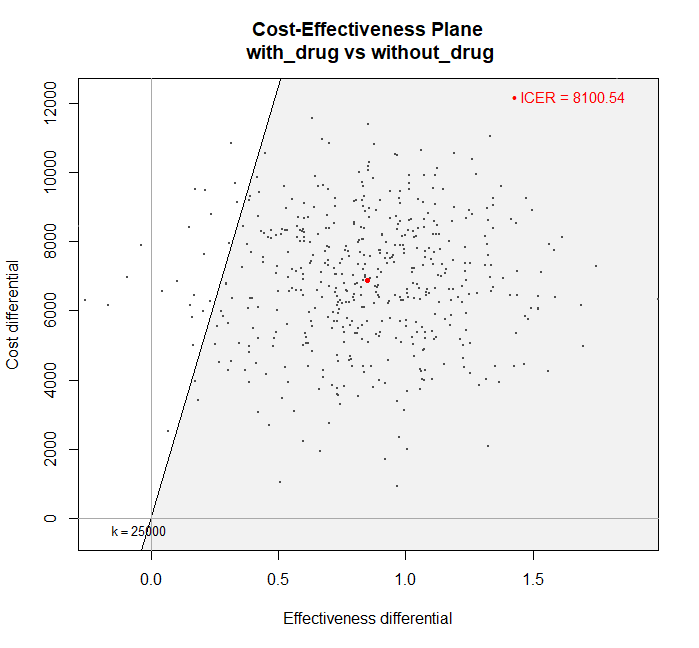
\includegraphics[scale=0.8]{ceplane_bcea}


\end{document}
